\section{Mathematical Formulation}
\label{sec:mathematical}
To study the spread of news in the population, three types of agents are considered: individuals (often referred to as "people"), \textit{real} news sources, and \textit{fake} news sources. In the context of this research, we define a real news source as a source which does its best effort to spread reliable, neutral and fact-checked information. Its opposite, the fake news source, has interest in spreading false information and actively and purposely does it. An example of one such network can be seen in Figure~\ref{pics:network_example}.

\begin{figure}
\centering
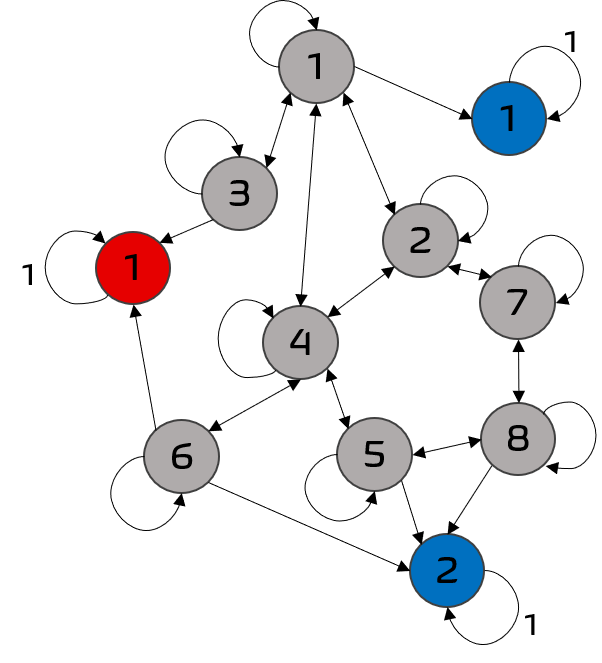
\includegraphics[width=2.5in]{Figures/network_example.png}
\caption{Example of one network that could be generated with our model. The network is formed by eight individuals, one source of fake news (red), two sources of real news (blue), and the links between nodes. Every node has a self loop, with weight 1 for the news sources, and the news sources only have. }
\label{pics:network_example}
\end{figure}
In order to be able to use a multitude of theoretical and analytical tools learned during the course, a linear model with the following update equation is studied
\begin{equation}
x(k+1) = A x(k),
\end{equation}
$x_i(k) \in [-1;1]$ represent the opinion of individual $i$ at timestep $k$ and $A$ is the adjacency matrix of the network, as in the popular opinion model\cite{Friedkin1990}.
Constructing the adjacency matrix $A$ is a non-trivial task as it requires several assumptions on the the existence of links between people, the existence of links between people and news sources, and the importance of each such link.
The existence of links between different individuals and between individuals and sources is determined either by their physical distance or randomly, as will be explained in more detail at a later stage.
To compute the weights in the adjacency matrix, several qualitative but sensible (in the authors' opinions) assumptions are made:
\renewcommand{\theenumi}{\roman{enumi}}
\begin{enumerate}
\item \textit{Similarity}: weights between similar people are stronger. This derives from the fact that people tend to listen to their peers, friends and colleagues more than people that are completely different from them. Real-world concepts that define similarity may include, but is not limited to: career path, certain behavorial traits, age, nationality, etc.
\item \textit{Influenceability}: different people give different importance to their own personal opinions and can be more or less influenced by external opinions.
\item \textit{Critical thinking}: depending on how developed the critical thinking ability of a person is, he/ she may believe \textit{news sources} more or less.
\end{enumerate}
Mathematically, 
Translating these assumptions into a network adjacency matrix $A$ can be done in multiple ways. In this research we mainly present one way and a second slightly modified to investigate opinion polarization. 
\subsection{Population Matrix}
To build a realistic network, the individuals can not be exactly the same. To differentiate between individuals, a \textit{population vector} $P \in {[0,1]}^{N \times t}$ is introduced, where $N$ is the number of individuals in the network and $t$ is the number characteristics defined for each person. In this research, $t=3$ and the chosen characteristics are similarity, influenceability and critical thinking ability. The position of an individual inside the matrix $P$ matters, as can be seen in Subsection \textbf{[Riferimento a subsubsection di Connections BEtween Individuals]}
\subsection{News Sources}
The number of news sources in the model is an important parameter when creating the network. We define the number of real news sources $N_{\text{real}}$ and the number of fake news sources $N_{\text{fake}}$.
\subsection{Existence of Connections}
When generating the adjacency matrix, connections between individuals and news sources need to be created.
\subsubsection{Connections Between Individuals}
Between individuals, the connections are created based on geographical distance. The real-world is simplified to a straight line with periodic boundaries, as can be seen in Figure ~ \textbf{(FAI FIGURE)}.
\acomment{spiegare come viene creata A, param C, nroot, locality}


